% !TeX root = RJwrapper.tex
\title{boiwsa: An R Package for Seasonal Adjustment of Weekly Data}


\author{by Tim Ginker}

\maketitle

\abstract{%
This article introduces the R package boiwsa for the seasonal adjustment of weekly data based on the discounted least squares method. It provides a user-friendly interface for computing seasonally adjusted estimates of weekly data and includes functions for creation of country-specific prior adjustment variables, as well as diagnostic tools to assess the quality of the adjustments. The utility of the package is demonstrated through two case studies: one based on US data of gasoline production characterized by a strong trend-cycle and dominant intra-yearly seasonality, and the other based on Israeli data of initial unemployment claims with two seasonal cycles (intra-yearly and intra-monthly) and the impact of two moving holidays.
}

\hypertarget{introduction}{%
\section{Introduction}\label{introduction}}

Policymakers and industry practitioners have long utilized weekly and other high-frequency data for timely updates on the state of various sectors of economic activity. Seasonal adjustment is a crucial component of this analysis as it facilitates the economic interpretation of data variations by allowing researchers to analyze these changes separately from the periodic fluctuations introduced by seasonal factors.

This article presents the R package \CRANpkg{boiwsa} for seasonal adjustment of weekly data based on the discounted least squares regression (DWR) introduced by Harrison and Johnston (1984). It provides a user-friendly interface for computing seasonally adjusted estimates of weekly data and includes functions for the creation of country-specific prior adjustment variables, as well as diagnostic tools to assess the quality of the adjustments. This equips practitioners with the ability to perform seasonal adjustments on their weekly data, thereby facilitating informed decision-making across a diverse array of applications.

Although attempts to develop procedures for the seasonal adjustment of weekly data date back to the early 20th century (Crum 1927), the volume of literature addressing this challenge remains relatively limited (for the latest review of the available methodology, see Proietti and Pedregal 2023). Moreover, while there has been notable growth in the number of high-frequency indicators requiring seasonal adjustment, the associated open-source software is less advanced and more intricate than the easily accessible and user-friendly tools commonly available for monthly and quarterly data (see Evans, Monsell, and Sverchkov 2021; R. J. Hyndman and Killick 2024).

The seasonal adjustment of high-frequency data presents multiple challenges due to its unique characteristics, which limit the straightforward application of conventional statistical methodologies. Most seasonal adjustment approaches generally encompass two primary steps: detrending and smoothing the cycle sub-series to compute the seasonal components. For instance, with monthly data, an initial application of a wide filter calculates and eliminates the trend. Subsequently, the detrended values are independently smoothed for each month, starting from January and progressing sequentially, to derive the seasonal components.

However, implementing a similar procedure on high-frequency data is not always feasible due to its potential for varying periodicity, presence of multiple seasonal cycles, and the moving window problem. For example, the number of weeks in a year varies between 52 and 53. Additionally, weekly data may exhibit multiple cycles, such as intra-monthly and intra-yearly patterns. As a result, commonly used methods like \texttt{X-13\ ARIMA-SEATS}, which work well for data with a single and fixed seasonal period, cannot be directly applied on weekly data.

To illustrate the challenge associated with the moving window problem, we constructed an artificial unobserved daily series underlying the observed weekly data. This synthetic daily data exhibits a simple monthly seasonal pattern characterized by a linear decrease from 100 to 0 over the course of a month. Consider the first six months of 2023, as depicted in Figure \ref{fig:mov-window-problem}. The black line represents the daily data, while, without loss of generality, each blue window corresponds to the first week of a month. Additionally, the green triangles denote the observed weekly averages derived from the black line. It becomes evident that each week aligns with a different portion of the intra-monthly cycle. As a result, even though the underlying daily seasonal pattern is constant, weekly aggregation produces a complex and evolving seasonality. Consequently, in this case, any method assuming a constant number of periods in a seasonal cycle and estimating a seasonal index for each would yield biased estimates.

\begin{figure}[H]

{\centering 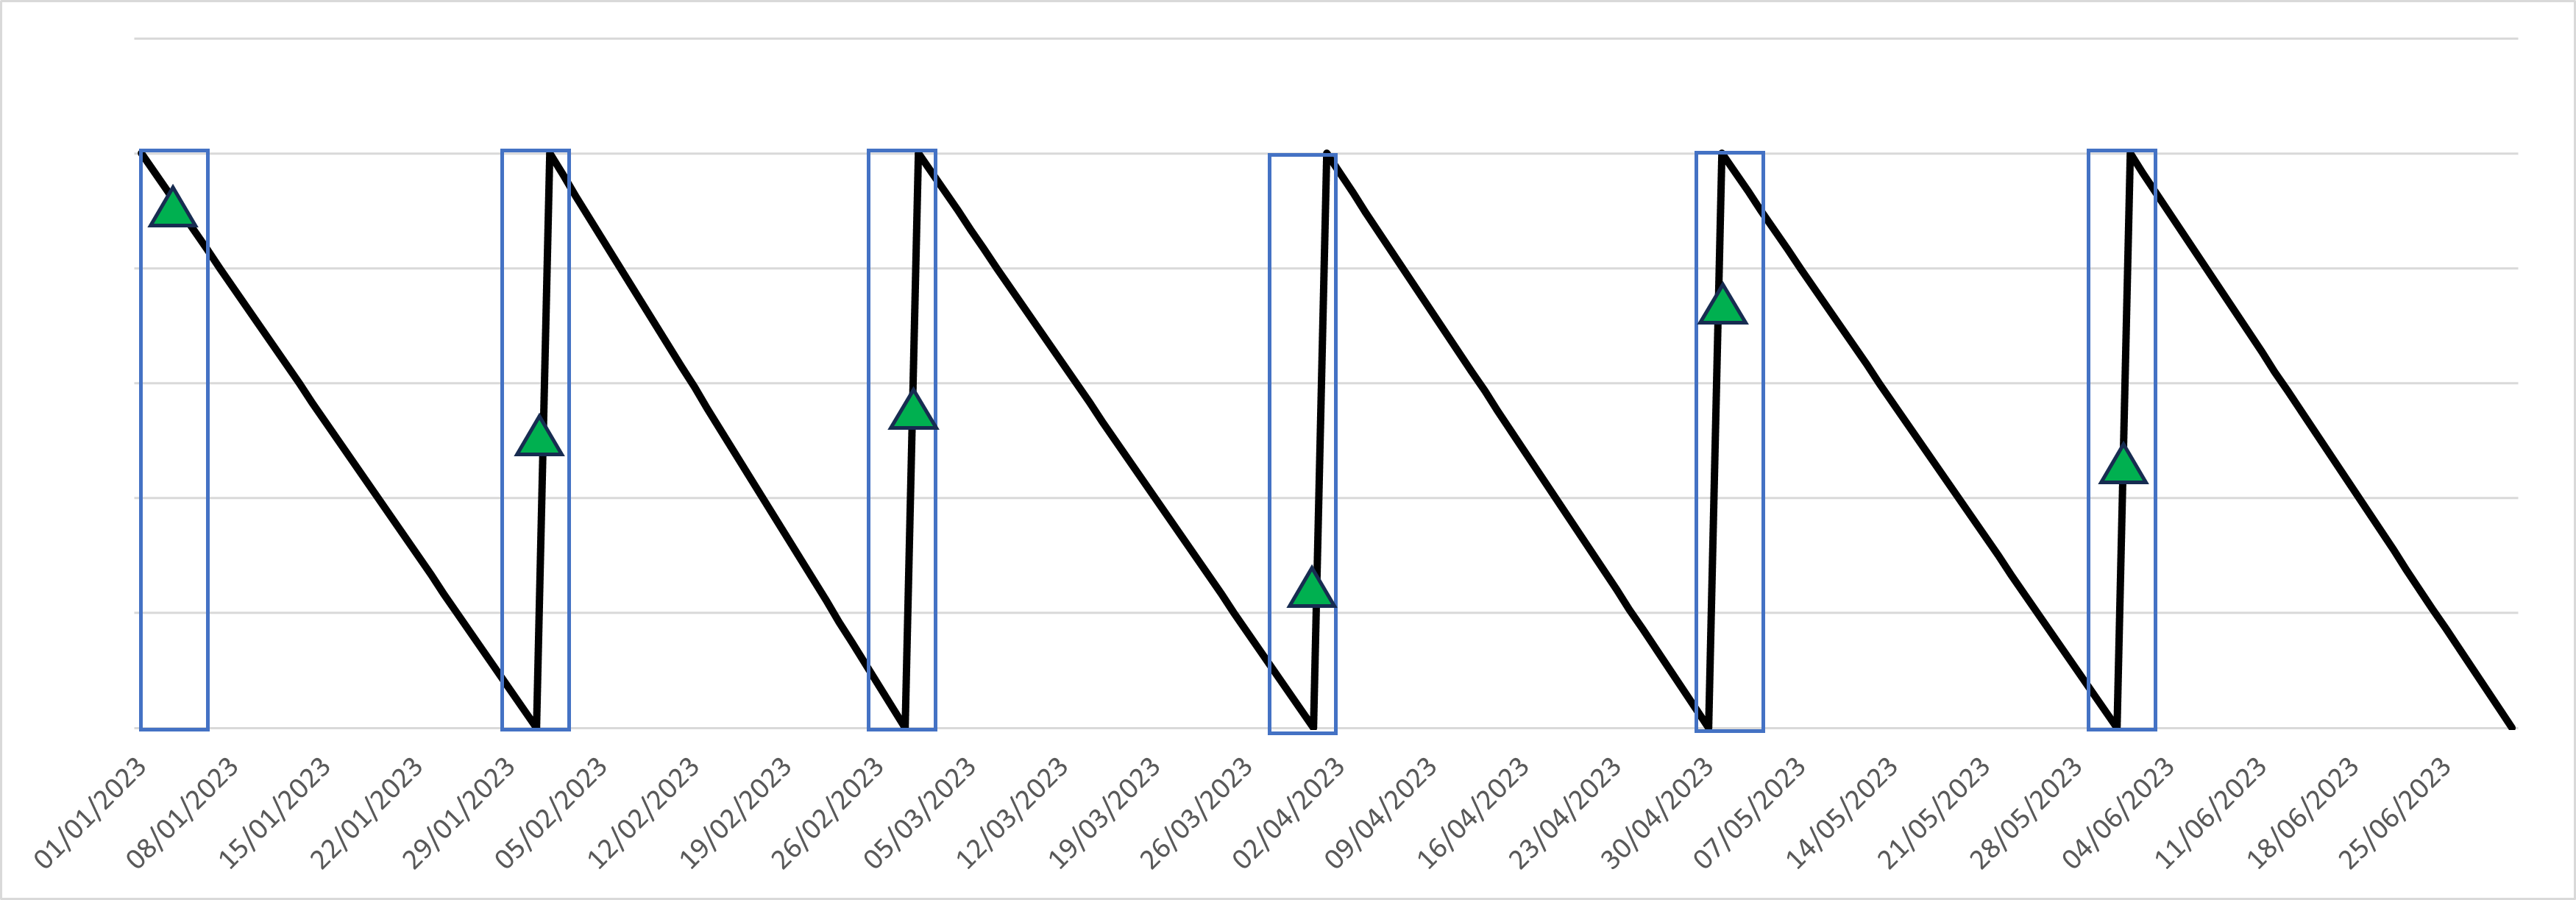
\includegraphics[width=1\linewidth,]{figures/mov-window-problem} 

}

\caption{Illustration of the moving window challenge.}\label{fig:mov-window-problem}
\end{figure}

Currently, a number of software tools for the seasonal adjustment of weekly data are in various stages of development. One such program is the \texttt{MoveReg} weekly seasonal adjustment method developed by the U.S. Bureau of Labor. This program can be executed using EViews or SAS, and its methodology is well documented and straightforward to implement. However, it is not available as open-source code. There are also some promising R packages currently under development, with the most advanced being \texttt{Ecce\ Signum} (McElroy and Livsey 2022)\footnote{The package is available on GitHub. See \url{https://github.com/tuckermcelroy/sigex}}. This package offers a method (in the Business Formation Statistics illustration) for the seasonal adjustment of weekly data that is based on the fractional airline model (FAM). However, it is worth mentioning a number of limitations associated with the aforementioned implementation of FAM. First, it implicitly assumes that the data must be differenced to eliminate a trend, which may not necessarily be present in the data. Second, similar to \texttt{MoveReg}, it is tailored to handle solely the intra-yearly cycle, a characteristic that could potentially restrict its applicability to data characterized by a substantial intra-monthly cycle, as presented in the application to the weekly unemployment claims in Israel.

Other software programs, occasionally employed for the seasonal adjustment of weekly data, rely on the Seasonal-Trend decomposition using Loess (STL), developed by R. B. Cleveland et al. (1990). A recent extension by Bandara, Hyndman, and Bergmeir (2024) introduced the concept of Multiple Seasonal-Trend decomposition using Loess (MSTL), thereby extending its application to time series featuring multiple seasonal cycles. It's important to note that both STL and MSTL decompositions are fundamentally based on the cycle subseries smoothing. They assume a constant number of seasonal factors in each cycle, and thus are unable to address the moving window problem discussed earlier. Additionally, these methods lack the capability to effectively account for trading day and moving holiday effects.

Finally, several studies suggest the utilization of forecasting models for the decomposition of time series, such as Prophet (Taylor and Letham 2018) or TBATS (De Livera, Hyndman, and Snyder 2011). However, these methods have been observed to yield less accurate decompositions (Bandara, Hyndman, and Bergmeir 2024).

The paper is organized as follows. Section 2 outlines our methodology. In Section 3, we provide examples of how to use the \CRANpkg{boiwsa} package, which is illustrated through two cases. The first example is based on US gasoline production data, which exhibits a strong trend-cycle and dominant intra-yearly seasonality. The second example is based on Israeli data of initial unemployment claims, where the level is relatively stable, but there are two seasonal cycles - intra-yearly and intra-monthly - and a pronounced effect of two moving holidays. 4 concludes.

\hypertarget{methodology}{%
\section{Methodology}\label{methodology}}

In this section, we describe our methodology. Our approach aligns closely with the locally-weighted least squares procedure introduced by W. P. Cleveland, Evans, and Scott (2014) that is implemented in the \texttt{MoveReg} program, albeit with several adjustments. First, in order to simplify the adjustment process, and facilitate automation, instead of first-differencing, we opt to extract the trend component using Friedman's SuperSmoother, implemented through the \texttt{stats::supsmu()} function (R Core Team 2024). Second, we incorporate a variation of DWR to enable the seasonal component to evolve dynamically over time. Unlike the weight structure proposed by W. P. Cleveland, Evans, and Scott (2014), our DWR implementation involves a single hyperparameter controlling the weight decay rate. In addition, DWR can be modified so that a different discount factor is applied to each model parameter. Although it is reasonable for weekly data to use the same discount factor for all parameters, future applications on higher frequency data could benefit from allowing each seasonal component to evolve at a different speed.

We consider the following decomposition model of the observed series \(y_{t}\):

\begin{equation}
    y_{t}=T_{t}+S_{t}+H_{t}+O_{t}+I_{t},
     \label{eq:eq1}
\end{equation}

where \(T_{t}\) represents the trend component, \(S_{t}\) the seasonal component, \(H_{t}\) the holiday and trading-day effects, \(O_{t}\) and \(I_{t}\) the outlier and irregular components respectively, and \(t\) denotes the date of the last day within a given week.

The seasonal component is specified using trigonometric variables as follows

\begin{eqnarray}
S_{t} &=&\sum_{k=1}^{K}\left( \alpha _{k}^{y}\sin (\frac{2\pi kD_{t}^{y}}{
n_{t}^{y}})+\beta _{k}^{y}\cos (\frac{2\pi kD_{t}^{y}}{n_{t}^{y}})\right) + \nonumber
\\
&&\sum_{l=1}^{L}\left( \alpha _{l}^{m}\sin (\frac{2\pi lD_{t}^{m}}{n_{t}^{m}}
)+\beta _{l}^{m}\cos (\frac{2\pi lD_{t}^{m}}{n_{t}^{m}})\right) ,
\label{eq:seqscomp}
\end{eqnarray}

where \(K\) and \(L\) define the number of yearly and monthly pairs of trigonometric variables, \(D_{t}^{y}\) and \(D_{t}^{m}\) are the day of the year and the day of the
month, and \(n_{t}^{y}\) and \(n_{t}^{m}\) are the number of days in the given
year or month\footnote{Note that \(n^y_t\) is either 365 or 366, depending on leap year, and that \(n^m_t\) is either 28, 29, 30, or 31.} (Pierce, Grupe, and Cleveland 1984). Thus, the seasonal adjustment procedure takes into account the existence of two cycles, namely intra-yearly and intra-monthly.

Similarly to the \texttt{X-11} method (Ladiray and Quenneville 2001), our procedure employs an iterative approach to estimate the different components. The seasonal adjustment algorithm comprises eight steps, which are detailed below:

\begin{itemize}
\item
  Step 1: Estimation of trend (\(T_{t}^{(1)}\)) using \texttt{stats::supsmu()}.
\item
  Step 2: Estimation of the Seasonal-Irregular component:
\end{itemize}

\begin{equation*}
    y_{t}-T_{t}^{(1)}=S_{t}+H_{t}+O_{t}+I_{t}.
\end{equation*}

\begin{itemize}
\item
  Step 2* (Optional): Searching for additive outliers using the method proposed by Findley et al. (1998).
\item
  Step 2** (Optional): Identifying the optimal number of trigonometric variables in \eqref{eq:seqscomp}.
\item
  Step 3: Calculation of seasonal factors, along with other potential factors such as \(H_{t}\) or \(O_{t}\), is done through DWR on the seasonal-irregular component extracted in Step 2. In this application, the discounting rate decays over the years. For each year \(t\) and the observed year \(\tau\), a geometrically decaying weight function is represented as: \(w_{t}=r^{|t-\tau|}\), where \(r \in (0,1]\). Several important points are worth mentioning. First, when \(r=1\), the method simplifies to ordinary least squares regression with constant seasonality. On the contrary, smaller values of \(r\) permit a more rapid rate of change in the seasonal component. However, it is advised against setting it below 0.5 to prevent overfitting. In addition, the choice of \(r\) affects the strength of revisions in the seasonally adjusted data, with higher values of \(r\) leading to potentially stronger revisions. Second, our methodology differs from the conventional one-way discounting, enabling the inclusion of future observations in the computation of seasonal factors. This approach circumvents the limitations of the forecasting methods discussed in Bandara, Hyndman, and Bergmeir (2024). Finally, the choice of year-based discounting is driven by the fact that in traditional discount-weighted regression, even with a conservative choice of \(r=0.95\), in weekly data, observations separated by more than 2 years would carry nearly negligible weight. Therefore, the use of year-based discounting prevents an overly rapid decay which may potentially lead to unstable estimates of the seasonal component.
\item
  Step 4: Estimation of the trend (\(T_{t}^{(2)}\)) from the seasonally and outlier adjusted series using \texttt{stats::supsmu()}.
\item
  Step 5: Estimation of the Seasonal-Irregular component:
  \[y_{t}-T_{t}^{(2)}=S_{t}+H_{t}+O_{t}+I_{t}\]
\item
  Step 6: Computing the final seasonal factors (and possibly other factors such as \(H_{t}\) or \(O_{t}\)) using DWR, as in step 3.
\item
  Step 7: Estimation of the final seasonally adjusted series:
  \[y_{t}-S_{t}-H_{t}\]
\item
  Step 8: Computing the final trend (\(T_{t}^{(3)}\)) estimate from the seasonally and outlier adjusted series using \texttt{stats::supsmu()}.
\end{itemize}

\hypertarget{use-of-boiwsa}{%
\section{Use of boiwsa}\label{use-of-boiwsa}}

In this section, we illustrate the use of our package and its key functionalities through two examples\footnote{The example code utilizes \CRANpkg{dplyr} (Wickham et al. 2023), \CRANpkg{ggplot2} (Wickham et al. 2024), and \CRANpkg{gridExtra} (Auguie 2017)}. The package is available on GitHub\footnote{See \url{https://github.com/timginker/boiwsa}}, and via the Comprehensive R Archive Network (CRAN)\footnote{See \url{https://cran.r-project.org/package=boiwsa}}. The first example is based on the data with a strong trend-cycle and dominant intra-yearly seasonality. The second example is based on the data where the level is relatively stable, but there are two seasonal cycles - intra-yearly and intra-monthly - and a pronounced effect of two moving holidays.

\hypertarget{example-1-gasoline-production-in-the-us}{%
\subsection{Example 1: Gasoline production in the US}\label{example-1-gasoline-production-in-the-us}}

Our first example uses the data on US finished motor gasoline product copied from the \CRANpkg{fpp2} package (R. Hyndman 2023), which is presented in Figure \ref{fig:gasoline} below. For convenience, it is stored as a \texttt{data.frame} with two columns: one with the series to be adjusted, stored as a numeric vector, and the second with the dates stored as a vector of class \texttt{Date}.

\begin{verbatim}
library(dplyr)
library(ggplot2)
library(boiwsa)

ggplot() +
  geom_line(
    aes(
      x = gasoline.data$date,
      y = gasoline.data$y
    ),
    color = "royalblue"
  ) +
  theme_bw() +
  ylab("Barrels per day (millions)") +
  xlab("Year")
\end{verbatim}

\begin{figure}[H]

{\centering \includegraphics[width=0.7\linewidth,]{boiwsa-paper_files/figure-latex/gasoline-1} 

}

\caption{Weekly gasoline production in the US, February 2, 1991 to January 20, 2017.}\label{fig:gasoline}
\end{figure}

Once users have their data loaded, they can use the \texttt{boiwsa} function to perform weekly seasonal adjustment. The following code shows the application of the package using automatic model selection.

\begin{verbatim}
res <- boiwsa(
  x = gasoline.data$y,
  dates = gasoline.data$date
)
\end{verbatim}

In general, the procedure can be applied with minimum interventions and requires only the series to be adjusted (\texttt{x} argument) and the associated dates (\texttt{dates} argument) provided in a date format. Unless specified otherwise (i.e., \texttt{my.k\_l\ =\ NULL}), the procedure automatically identifies the best number of trigonometric variables in \eqref{eq:seqscomp} to model the intra-yearly (\(K\)) and intra-monthly (\(L\)) seasonal cycles based on the Akaike Information Criterion corrected for small sample sizes (AICc). The information criterion can be adjusted through the \texttt{ic} option. Like other software, there are three options: ``aic'', ``aicc'', and ``bic''. The weighting decay rate is specified by \texttt{r}. By default \(r=0.8\) which is similar to what is customary in the literature (Harvey 1990). For the full list of arguments and their description, see Table \ref{tab:inputs-tex} below.

\begin{table}[H]
\centering
\caption{\label{tab:inputs-tex}Input arguments for boiwsa}
\centering
\resizebox{\ifdim\width>\linewidth\linewidth\else\width\fi}{!}{
\fontsize{7}{9}\selectfont
\begin{tabular}[t]{ll}
\toprule
Input argument & Description\\
\midrule
x & Numeric vector with series to be seasonally adjusted\\
dates & Vector of class "Date", containing the data dates\\
r & Defines the rate of decay of the weights. Should be between zero and one. By default is set to 0.8\\
auto.ao.search & Boolean. Search for additive outliers\\
out.threshold & t-statistic threshold in outlier search. By default is set to 3.8 as suggested by Findley (1998)\\
\addlinespace
ao.list & Vector with user-specified additive outliers in a date format\\
my.k\_l & Numeric vector defining the number of yearly and monthly trigonometric variables. If NULL, is found automatically using the information criteria (AICc)\\
H & Matrix with holiday/working day factors or other user-defined preadjustments\\
ic & Information criterion used in the automatic search for the number of trigonometric regressors. There are three options: aic, aicc, and bic. aicc is set as default\\
method & Decomposition type: additive or multiplicative (log transformation)\\
\bottomrule
\end{tabular}}
\end{table}

\FloatBarrier

\FloatBarrier

In addition, the procedure automatically searches for additive outliers (AO) using the method described in Appendix C of Findley et al. (1998). To disable the automatic AO search, set \texttt{auto.ao.search\ =\ F}. To add user-defined AOs, use the \texttt{ao.list} option. As suggested by Findley et al. (1998), the t-statistic threshold for outlier search is by default set to \(3.8\). However, since high-frequency data are generally more noisy (Proietti and Pedregal 2023), it could be advantageous to consider setting a higher threshold by adjusting the \texttt{out.threshold} argument.

The \texttt{boiwsa} function returns a list object containing the results. The seasonally adjusted series is stored in a vector called \texttt{sa}. The estimated seasonal factors are stored as \texttt{sf}. In addition, the user can see the number of trigonometric terms chosen in automatic search (\texttt{my.k\_l}) and the position of additive outliers (\texttt{ao.list}) found by the automatic routine. For the full list of outputs and their description, see Table \ref{tab:values-tex}.

\FloatBarrier
\begin{table}[H]
\centering
\caption{\label{tab:values-tex}Output values for boiwsa}
\centering
\resizebox{\ifdim\width>\linewidth\linewidth\else\width\fi}{!}{
\fontsize{7}{9}\selectfont
\begin{tabular}[t]{ll}
\toprule
Value & Description\\
\midrule
sa & Numeric vector with seasonally adjusted series\\
x & Numeric vector with series to be seasonally adjusted\\
my.k\_l & Number of trigonometric variables used to model the seasonal pattern\\
sf & Estimated seasonal effects. Note that these contain the seasonal effects represented by the trigonometric variables as well as the user-defined preadjustments in H\\
hol.factors & Estimated holiday effects or other user-defined variables supplied in H\\
\addlinespace
out.factors & Estimated outlier effects\\
beta & DWR coefficients for the last year\\
trend & Final trend estimate (T\_t\textasciicircum{}(3))\\
ao.list & Additive outlier dates\\
m & lm object. Unweighted OLS regression on the full sample\\
\bottomrule
\end{tabular}}
\end{table}
\FloatBarrier

After the seasonal adjustment, we can plot the adjusted data to visualize the seasonal pattern:

\begin{verbatim}
plot(res)
\end{verbatim}

\begin{figure}[H]

{\centering \includegraphics[width=0.7\linewidth,]{boiwsa-paper_files/figure-latex/gasoline-sa-1} 

}

\caption{Weekly gasoline production in the US, February 2, 1991 to January 20, 2017.}\label{fig:gasoline-sa}
\end{figure}

To assess the quality of the adjustment, we can plot the autoregressive spectrum of the original and seasonally adjusted data, as illustrated in the code below:

\begin{verbatim}
# spectrum of the original series (after detrending)
spec0 <- spec.ar((res$x - res$trend), order = 60, plot = F)
# spectrum of the seasonally adjusted series (after detrending)
spec1 <- spec.ar((res$sa - res$trend), order = 60, plot = F)

# plot
ggplot() +
  geom_line(aes(x = spec0$freq, y = spec0$spec, color = "orig")) +
  geom_line(aes(x = spec0$freq, y = spec1$spec, color = "sa")) +
  geom_vline(xintercept = 1:2 / 4.34, linetype = "dashed") +
  geom_text(aes(x = 1:2 / 4.34, label = "
 Intra-monthly cycle peaks", y = 0.5 * max(spec0$spec)), colour = "black", angle = 90) +
  geom_vline(xintercept = (1:3) / 52.1775, linetype = "dashed") +
  geom_text(aes(x = 3 / 52.1775, label = "
 First three intra-yearly cycle peaks", y = 0.5 * max(spec0$spec)), colour = "black", angle = 90) +
  scale_color_manual(
    name = "",
    values = c("orig" = "#31a354", "sa" = "#3182bd"),
    labels = c("Original", "Seasonally adjusted")
  ) +
  theme_bw() +
  theme(legend.position = "bottom") +
  theme(legend.text = element_text(size = 11)) +
  ylab(" ") +
  xlab("Frequency")
\end{verbatim}

\begin{figure}[H]

{\centering \includegraphics[width=0.7\linewidth,]{boiwsa-paper_files/figure-latex/gasoline-spec-1} 

}

\caption{Autoregressive spectrum of weekly gasoline production in the US.}\label{fig:gasoline-spec}
\end{figure}

In spectral analysis, it is customary to remove the trend component prior to conducting the analysis. This step prevents the trend from obscuring the peaks associated with the seasonal component. If this pre-processing step is omitted, particularly in a time series with a strong trend, the resulting spectrum will predominantly display peaks at the beginning of the axes, thereby complicating the identification of seasonal peaks. Additionally, to compute the spectrum, the number of lags is set to 60. Finally, the first three yearly cycle peaks and the two monthly peaks are marked using vertical lines. Figure \ref{fig:gasoline-spec}, which can also be generated using \texttt{boiwsa::plot\_spec}, illustrates that the series originally had a single intra-yearly seasonal cycle, but this component was completely removed by the procedure.

We can also inspect the output to check if the number of trigonometric terms chosen by the automatic procedure matches our visual findings:

\begin{verbatim}
print(res)
\end{verbatim}

\begin{verbatim}
#> 
#>  number of yearly cycle variables:  12 
#>  number of monthly cycle variables:  0 
#>  list of additive outliers:  1998-03-28
\end{verbatim}

As can be seen, the number of yearly terms, \(K\), is 12 and the number of monthly terms is zero, which is consistent with the observed spectrum.

\hypertarget{example-2-initial-unemployment-claims-in-israel}{%
\subsection{Example 2: Initial unemployment claims in Israel}\label{example-2-initial-unemployment-claims-in-israel}}

In this subsection, we present our second example that is based on Israeli data. The data has no obvious trend but has two pronounced seasonal cycles, intra-yearly and intra-monthly. Moreover, there is a strong impact of two moving holidays and a working day effect.

The series under consideration is the weekly number of initial registrations at the Israeli Employment Service. Due to a prolonged period of structural change associated with the COVID-19 crisis, we limit our sample to January 11, 2014, to January 4, 2020. It is worth noting that addressing such events in the context of high-frequency data presents a significant challenge. Furthermore, given the duration of the COVID-19 crisis, the standard methods of incorporating outlier variables, which are also available in our package, appear to be incapable of providing a satisfactory solution in this context.

Registration and reporting at the Employment Service are mandatory prerequisites for individuals seeking to receive an unemployment benefit. Therefore, applicants are expected to register promptly after their employment has been terminated. Given that most employment contracts conclude toward the end of the month, an increased number of applications is anticipated at the beginning of the month, leading to an intra-monthly seasonal pattern. Additionally, as can be seen in Figure \ref{fig:unemp} below, on an annual basis, three distinct peaks are observed, with the final one occurring in August. This peak is closely tied to seasonal workers, leading to the creation of an intra-yearly cycle.

\begin{figure}[H]

{\centering \includegraphics[width=0.7\linewidth,]{boiwsa-paper_files/figure-latex/unemp-1} 

}

\caption{Weekly number of initial unemployment claims in Israel, January 11, 2014 to January 4, 2020.}\label{fig:unemp}
\end{figure}

Furthermore, each year, there are two weeks in which the activity plunges to nearly zero due to the existence of two moving holidays associated with Rosh Hashanah and Pesach. Moreover, a working day effect is expected, which leads to a reduced number of applications in weeks with fewer working days. These effects are captured and modeled through additional variables generated by the dedicated functions in \CRANpkg{boiwsa}.

To generate a working day variable, we use the \texttt{boiwsa::simple\_td} function, designed to aggregate the count of full working days within a week and normalize it. This function requires two parameters: the data dates and a \texttt{data.frame} object containing information about working days. The \texttt{data.frame} should be in a daily frequency and contain two columns: ``date'' and ``WORKING\_DAY\_PART''. For a complete working day, the ``WORKING\_DAY\_PART'' column should be assigned a value of 1, for a half working day 0.5, and for a holiday, the value should be set to 0.

Moving holiday variables can be created using the \texttt{boiwsa::genhol} function. These variables are computed using the Easter formula in Table 2 of Findley et al. (1998), with the calendar centering to avoid bias, as indicated in the documentation. In the present example, the impact of each holiday is concentrated within a single week, resulting in a noticeable drop and subsequent increase in the number of registrations during the following week. To account for this effect, we employ dummy variables that are globally centered. These dummy variables are created using a custom function - \texttt{boiwsa::my\_rosh}, which is created for this illustrative scenario.

The code below illustrates the entire process based on the \texttt{boiwsa::lbm\ dataset}: creation of working day adjustment variables using the \texttt{boiwsa::simple\_td} function; creation of moving holiday variables using the dedicated functions, and adding the combined input into the \texttt{boiwsa::boiwsa} function.

\begin{verbatim}
# creating an input for simple_td 
dates_il %>%
  select(DATE_VALUE, ISR_WORKING_DAY_PART) %>%
  `colnames<-`(c("date", "WORKING_DAY_PART")) %>%
  mutate(date = as.Date(date)) -> df.td
# creating a matrix with a working day variable
td <- simple_td(dates = lbm$date, df.td = df.td)

# generating the Rosh Hashanah and Pesach moving holiday variables
rosh <- my_rosh(
  dates = lbm$date,
  holiday.dates = holiday_dates_il$rosh
)
# renaming (make sure that all the variables in H have distinct names)
colnames(rosh) <- paste0("rosh", colnames(rosh))

pesach <- my_rosh(
  dates = lbm$date,
  holiday.dates = holiday_dates_il$pesah,
  start = 3, end = -1
)
colnames(pesach) <- paste0("pesach", colnames(pesach))


# combining the prior adjustment variables in a single matrix
H <- as.matrix(cbind(rosh[, -1], pesach[, -1], td[, -1]))
# running seasonal adjustment routine
res <- boiwsa(
  x = lbm$IES_IN_W_ADJ,
  dates = lbm$date,
  H = H,
  out.threshold = 3.8
)
\end{verbatim}

Subsequently, we can visually examine the results of the procedure presented in Figure \ref{fig:unemp-sa-bad} below:

\begin{verbatim}
plot(res)
\end{verbatim}

\begin{figure}[H]

{\centering \includegraphics[width=0.7\linewidth,]{boiwsa-paper_files/figure-latex/unemp-sa-bad-1} 

}

\caption{Weekly number of initial unemployment claims in Israel: Original, Seasonally adjusted, and the decomposition with `out.threshold=3.8`.}\label{fig:unemp-sa-bad}
\end{figure}

As we can see in the plot, the procedure has successfully eliminated the annual and monthly seasonal cycles, along with the influences of moving holidays. Nevertheless, it's notable that a few pronounced declines emerge in the seasonally adjusted series from 2016 onward. As previously mentioned, weekly data often contain more noise, potentially prompting the inclusion of outlier variables where they might not be necessary. This inclusion could introduce bias to the seasonal component, consequently leading to the observed distortions.

While the suitability of the approach depends on the specific application, it appears that the recommended outlier threshold of 3.8, typically suggested for monthly data, might be insufficiently conservative for the weekly series. Consequently, a careful examination of the identified outliers is strongly advised. To tackle this issue, one possible solution involves raising the \texttt{out.threshold}, as demonstrated in the code and Figure summarizing the results below.

\begin{verbatim}
res <- boiwsa(
  x = lbm$IES_IN_W_ADJ,
  dates = lbm$date,
  H = H,
  out.threshold = 5
)
\end{verbatim}

\begin{verbatim}
plot(res)
\end{verbatim}

\begin{figure}[H]

{\centering \includegraphics[width=0.7\linewidth,]{boiwsa-paper_files/figure-latex/unemp-sa-fixed-1} 

}

\caption{Weekly number of initial unemployment claims in Israel: Original, Seasonally adjusted, and the decomposition with `out.threshold=5`.}\label{fig:unemp-sa-fixed}
\end{figure}

Following a thorough visual examination of the seasonally adjusted data, we can now move forward with the spectrum diagnostics. As illustrated in Figure \ref{fig:unemp-spec} below, corroborating our initial analysis of potential underlying seasonal patterns, it becomes evident that the data has two distinct seasonal cycles. Additionally, it is noteworthy that our procedure successfully removed the corresponding peaks, thereby highlighting its effectiveness.

\begin{verbatim}
plot_spec(res)
\end{verbatim}

\begin{figure}[H]

{\centering \includegraphics[width=0.7\linewidth,]{boiwsa-paper_files/figure-latex/unemp-spec-1} 

}

\caption{Autoregressive spectrum of a weekly number of initial unemployment claims in Israel.}\label{fig:unemp-spec}
\end{figure}

\hypertarget{summary}{%
\section{Summary}\label{summary}}

The package \CRANpkg{boiwsa} is developed to equip practitioners with the ability to perform seasonal adjustments on the weekly data, thereby facilitating informed decision-making across a diverse array of applications. It provides a user-friendly interface for computing seasonally adjusted estimates of weekly data and includes functions for the creation of country-specific prior adjustment variables, as well as diagnostic tools to assess the quality of the adjustments. The empirical applications presented in this paper demonstrate it's functionality and ability to perform under various practical scenarios.

\hypertarget{acknowledgments}{%
\section*{Acknowledgments}\label{acknowledgments}}
\addcontentsline{toc}{section}{Acknowledgments}

I would like to thank the editor and two anonymous referees for their remarks and suggestions that helped improve the paper and the package. I'm grateful to Karsten Webel for his review and advice. I would also like to thank Ariel Mantzura, Eyal Argov, Daniel Rosenman, and Ramsis Gara for their valuable suggestions and discussions. The views expressed in this paper are those of the author and do not necessarily reflect the views of the Bank of Israel.

\hypertarget{references}{%
\section*{References}\label{references}}
\addcontentsline{toc}{section}{References}

\hypertarget{refs}{}
\begin{CSLReferences}{1}{0}
\leavevmode\vadjust pre{\hypertarget{ref-gridExtra}{}}%
Auguie, Baptiste. 2017. \emph{{gridExtra}: Miscellaneous Functions for {``{Grid}''} Graphics}. \url{https://CRAN.R-project.org/package=gridExtra}.

\leavevmode\vadjust pre{\hypertarget{ref-bandara2021mstl}{}}%
Bandara, Kasun, Rob J Hyndman, and Christoph Bergmeir. 2024. {``{MSTL}: A Seasonal-Trend Decomposition Algorithm for Time Series with Multiple Seasonal Patterns.''} \emph{International Journal of Operational Research}.

\leavevmode\vadjust pre{\hypertarget{ref-cleveland1990stl}{}}%
Cleveland, Robert B, William S Cleveland, Jean E McRae, and Irma Terpenning. 1990. {``{STL}: A Seasonal-Trend Decomposition.''} \emph{Journal of Official Statistics} 6 (1): 3--73.

\leavevmode\vadjust pre{\hypertarget{ref-cleveland2014}{}}%
Cleveland, William P., Thomas D. Evans, and Stuart Scott. 2014. {``{Weekly Seasonal Adjustment - A Locally-weighted Regression Approach}.''} Economic Working Papers. Bureau of Labor Statistics.

\leavevmode\vadjust pre{\hypertarget{ref-crum1927}{}}%
Crum, W. L. 1927. {``Weekly Fluctuations in Outside Bank Debits.''} \emph{The Review of Economic Statistics} 9 (1): 30--36.

\leavevmode\vadjust pre{\hypertarget{ref-tbats}{}}%
De Livera, Alysha M, Rob J Hyndman, and Ralph D Snyder. 2011. {``Forecasting Time Series with Complex Seasonal Patterns Using Exponential Smoothing.''} \emph{Journal of the American Statistical Association} 106 (496): 1513--27. \url{https://doi.org/10.1198/jasa.2011.tm09771}.

\leavevmode\vadjust pre{\hypertarget{ref-evansreview}{}}%
Evans, Thomas D, Brian C Monsell, and Michae Sverchkov. 2021. {``{R}eview of {A}vailable {P}rograms for {S}easonal {A}djustment of {W}eekly {D}ata.''} In \emph{{P}roceedings of the {J}oint {S}tatistical {M}eetings}. American Statistical Association.

\leavevmode\vadjust pre{\hypertarget{ref-findley1998}{}}%
Findley, David F., Brian C. Monsell, William R. Bell, Mark C. Otto, and Bor-Chung Chen. 1998. {``New Capabilities and Methods of the {X}-12-ARIMA Seasonal-Adjustment Program.''} \emph{Journal of Business \& Economic Statistics} 16 (2): 127--52. \url{https://doi.org/10.2307/1392565}.

\leavevmode\vadjust pre{\hypertarget{ref-DWR}{}}%
Harrison, P. J., and F. R. Johnston. 1984. {``Discount Weighted Regression.''} \emph{The Journal of the Operational Research Society} 35 (10): 923--32. \url{https://doi.org/10.2307/2582135}.

\leavevmode\vadjust pre{\hypertarget{ref-harvey1990}{}}%
Harvey, Andrew C. 1990. \emph{Forecasting, Structural Time Series Models and the {K}alman Filter}. Cambridge University Press.

\leavevmode\vadjust pre{\hypertarget{ref-fpp2}{}}%
Hyndman, Rob. 2023. \emph{{fpp2}: {D}ata for "{F}orecasting: {P}rinciples and {P}ractice" (2nd {E}dition)}. \url{https://CRAN.R-project.org/package=fpp2}.

\leavevmode\vadjust pre{\hypertarget{ref-ts_task_view}{}}%
Hyndman, Rob J, and Rebecca Killick. 2024. \emph{{C}RAN {T}ask {V}iew: {T}ime {S}eries {A}nalysis}. \url{https://CRAN.R-project.org/view=TimeSeries}.

\leavevmode\vadjust pre{\hypertarget{ref-ladiray2001}{}}%
Ladiray, Dominique, and Benoit Quenneville. 2001. \emph{Seasonal Adjustment with the {X}-11 Method}. Springer New York, NY.

\leavevmode\vadjust pre{\hypertarget{ref-mcelroy2022}{}}%
McElroy, Tucker S, and James A Livsey. 2022. {``{Ecce Signum}: {An} {R} {P}ackage for Multivariate Signal Extraction and Time Series Analysis.''} \emph{arXiv Preprint arXiv:2201.02148}. \url{https://doi.org/10.48550/arXiv.2201.02148}.

\leavevmode\vadjust pre{\hypertarget{ref-Pierce_1984}{}}%
Pierce, David A., Michael R. Grupe, and William P. Cleveland. 1984. {``Seasonal Adjustment of the Weekly Monetary Aggregates: A Model-Based Approach.''} \emph{Journal of Business \& Economic Statistics} 2 (3): 260--70. \url{https://doi.org/10.2307/1391708}.

\leavevmode\vadjust pre{\hypertarget{ref-proietti2023seasonality}{}}%
Proietti, Tommaso, and Diego J Pedregal. 2023. {``Seasonality in {H}igh {F}requency {T}ime {S}eries.''} \emph{Econometrics and Statistics} 27: 62--82. \url{https://doi.org/10.1016/j.ecosta.2022.02.001}.

\leavevmode\vadjust pre{\hypertarget{ref-stats}{}}%
R Core Team. 2024. \emph{R: A Language and Environment for Statistical Computing}. Vienna, Austria: R Foundation for Statistical Computing. \url{http://www.R-project.org/}.

\leavevmode\vadjust pre{\hypertarget{ref-prophet}{}}%
Taylor, Sean J, and Benjamin Letham. 2018. {``Forecasting at Scale.''} \emph{The American Statistician} 72 (1): 37--45. \url{https://doi.org/10.7287/peerj.preprints.3190v2}.

\leavevmode\vadjust pre{\hypertarget{ref-ggplot2manual}{}}%
Wickham, Hadley, Winston Chang, Lionel Henry, Thomas Lin Pedersen, Kohske Takahashi, Claus Wilke, Kara Woo, et al. 2024. \emph{{ggplot2}: Create Elegant Data Visualisations Using the Grammar of Graphics}. \url{https://cran.r-project.org/package=ggplot2}.

\leavevmode\vadjust pre{\hypertarget{ref-dplyr}{}}%
Wickham, Hadley, Romain François, Lionel Henry, Kirill Müller, and Davis Vaughan. 2023. \emph{{dplyr}: A Grammar of Data Manipulation}. \url{https://CRAN.R-project.org/package=dplyr}.

\end{CSLReferences}


\address{%
Tim Ginker\\
Bank of Israel\\%
Bank of Israel. POB 780, 91007, Jerusalem, Israel\\
%
%
\textit{ORCiD: \href{https://orcid.org/0000-0002-7138-5417}{0000-0002-7138-5417}}\\%
\href{mailto:timginker@gmail.com}{\nolinkurl{timginker@gmail.com}}%
}
